\documentclass[11pt]{article}
\usepackage[margin=1in]{geometry}
\usepackage{amsmath,graphicx,booktabs,xcolor,hyperref}
\usepackage[skip=4pt]{caption}
\hypersetup{colorlinks=true,linkcolor=blue!55!black,urlcolor=blue!55!black}
\newcommand{\fig}[1]{\includegraphics[width=\linewidth]{figs/#1}}
\sloppy
\title{\textbf{The paper-correct HCAPO still drifts:}\\[3pt]
\large why a faithful implementation of Eq.~6--7 lengthens its own replies}
\author{Agentic-RL-CA project}
\date{2026-07-30}

\begin{document}
\maketitle

\begin{abstract}
\noindent This note is about \emph{one} run: HCAPO implemented exactly as the paper specifies
(arXiv:2603.08754, Eq.~6--7 --- verified: the credit ratio $\rho$ centred on 1.0, two-sided, clip
engaging on both ends). It trained cleanly for $\sim$150 steps, then its replies quadrupled in 40
steps and pinned against the 2048-token cap, with no accuracy gain. The drift is not our earlier
port bug (that was found and fixed first); it follows from two properties of the formulation
itself: (i) a turn's hindsight score is a \emph{per-token average}, which rises when a turn is
padded with easy filler --- an incentive we measure in healthy-length rollouts \emph{before any
drift exists} (Fig.~3); and (ii) the trajectory-average normalisation makes credit \emph{relative},
which cancels collective lengthening but not the batch-by-batch fact that the \emph{longer sibling
wins} --- so each update nudges the policy longer, permanently, while the normalisation guarantees
nobody ever nets credit from it (Fig.~2). The race only ends when padding has homogenised all turns
and the credit signal itself dies (Fig.~4).
\end{abstract}

\section{What happened}
\begin{figure}[h]\centering\fig{fig1_drift.pdf}
\caption{Top: average reply length. The paper-correct run behaves normally for $\sim$150 steps ---
indistinguishable from GRPO --- then drifts from $\sim$250 to $\sim$1{,}230 tokens between steps
160 and 200 and saturates against the cap. Bottom: accuracy over the same steps --- flat through
the entire drift, and never above plain GRPO.}
\end{figure}

We verified the implementation before this run: $\rho$ starts centred on $1.0$ (batch mean
$1.0006$), takes values on both sides of 1 (both clip bounds engage), and a unit test confirms
that lengthening \emph{all} turns together leaves $\rho$ exactly unchanged --- the invariance the
paper's intra-trajectory normalisation is designed to provide. The drift happened anyway.

\section{Why: the incentive exists before the drift}
HCAPO scores a turn by its \emph{average} per-token log-probability under a hindsight-augmented
prompt (Eq.~6), then credits each turn by its score \emph{relative to the trajectory's average}
(Eq.~7). Averages can be padded: the tokens that carry a turn's content are hard (low probability),
filler is easy (high probability), so adding filler raises the average. The question is whether
this bites \emph{in practice}, in the healthy regime, within Eq.~7's normalisation. We measured it
directly --- 145 healthy-length trajectories, every turn re-scored with and without the hindsight
text, everything compared \emph{within} its own trajectory:

\begin{figure}[h]\centering
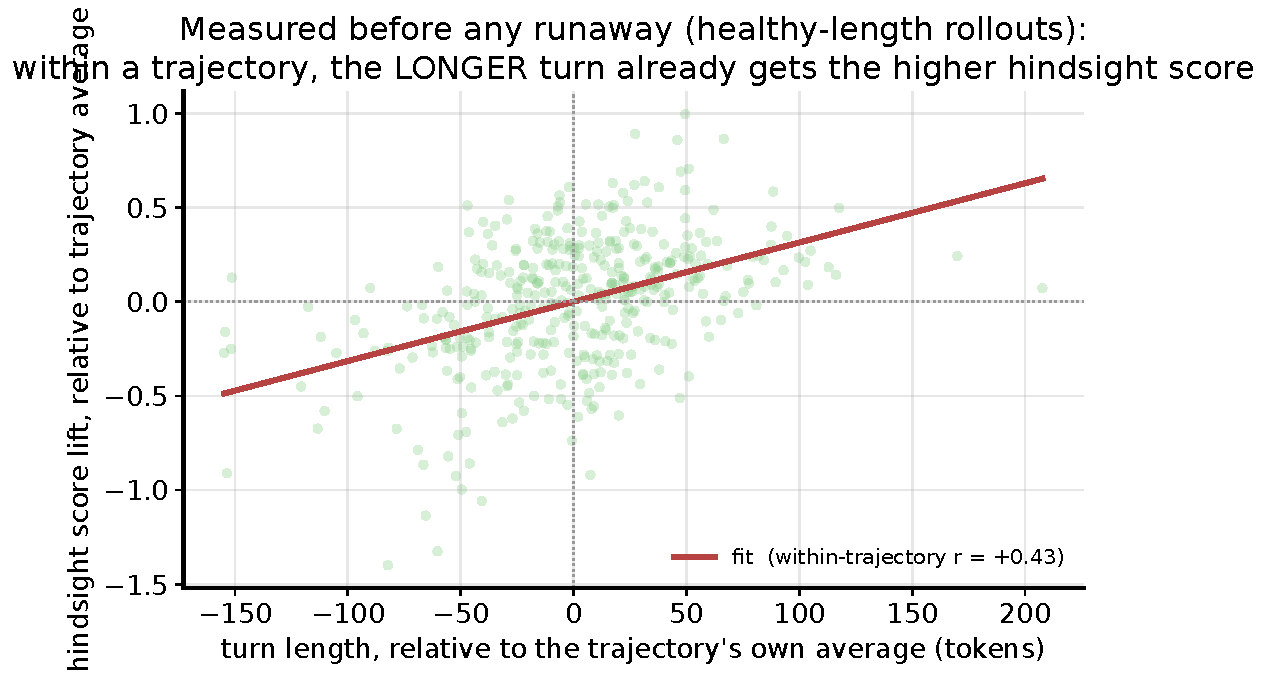
\includegraphics[width=0.78\linewidth]{figs/fig3_incentive.pdf}
\caption{Each point is one turn, positioned by how much longer it is than its trajectory's average
(x) and how much higher its hindsight score-lift is than the trajectory's average (y). The
correlation is $r=+0.43$ (and $+0.33$ after controlling for turn position): \textbf{before any
drift exists, the relatively longer turn already gets the relatively higher hindsight score.} This
is exactly the quantity Eq.~7 turns into credit.}
\end{figure}

\noindent Two details make this worse than a generic length bias. First, the plain (no-hindsight)
score shows \emph{no} such correlation ($r=-0.02$) --- the length preference is created by the
hindsight injection itself: appending the episode's final observation perturbs early tokens most,
and longer turns dilute that perturbation away. Second, it survives position controls, so it is
not an artifact of later turns being longer.

\section{Why the normalisation doesn't save you}
\begin{figure}[h]\centering\fig{fig2_ratchet.pdf}
\caption{The treadmill. In every batch, the turn that happens to be a little longer and more
padded than its trajectory-siblings gets $\rho>1$ and is reinforced (red). The policy shifts
longer \emph{everywhere}; the normalisation re-centres, so nobody keeps any credit advantage ---
but the behavioural update is permanent, and at the new, longer baseline the same comparison
favours the same thing. Grading on a curve does not stop grade inflation; it only guarantees the
inflation buys nothing.}
\end{figure}

The invariance argument (``if everyone lengthens together, $\rho$ is unchanged'') is true and we
verified it --- but training never moves in lockstep. Gradients act on \emph{individual sampled
turns}, and Fig.~3 shows which individual turns win: the longer ones. The uniform direction being
invariant means precisely that there is \emph{no restoring force}: collective lengthening is free.
Relative credit plus an absolute lever (padding raises your own score) is an arms race.

\section{How it ends: the signal eats itself}
\begin{figure}[h]\centering\fig{fig4_signal.pdf}
\caption{Top: the batch \emph{mean} of $\rho$ is pinned at 1.0 by construction throughout ---
monitoring the mean can never see this failure. Bottom: the \emph{spread} of $\rho$ --- the
method's entire information content --- collapses from 0.135 to 0.030 exactly across the drift
window. As padding homogenises the turns, every turn's average score converges to the same generic
fluency level, all credit ratios approach 1, and the hindsight term goes silent. What remains is
plain GRPO plus a small position bonus, at $\sim$12$\times$ the token cost.}
\end{figure}

\noindent The endpoint is self-limiting rather than catastrophic: accuracy holds around
0.38--0.42 while more than half of all turns are cut off mid-sentence by the cap, and each
training step takes $\sim$2.6$\times$ longer than before the drift.

\section*{What would actually fix it}
(1) Score turns on a \emph{fixed window} or another length-robust statistic, so filler cannot move
the score --- this removes the lever the ratchet needs. (2) Exclude the final (answer) turn from
hindsight credit; separate measurements show it is the top-credit turn in 73\% of healthy-regime
trajectories purely because the ending entails it. (3) A per-turn length penalty would mask the
symptom but leave the mis-scoring in place.

\section*{Fine print}
One seed; SearchQA (Qwen3-4B, non-thinking, 4-turn episodes, 2048-token cap). The paper's own
benchmarks (ALFWorld, WebShop) use short action-style turns under tight caps and may never enter
this regime; this note is a claim about the formulation on this task class, not a refutation of
the paper's results. The run is still training; step-500 finals will be appended. Companion
documents: the full-family runaway report (\texttt{2026-07-30\_hcapo\_length\_runaway/}), the
technical implementation note (\texttt{2026-07-29\_hcapo\_implementation\_note/}), and the
timestamped prediction/retraction trail
(\texttt{2026-07-21\_4b\_horizon\_eval/results/hcapo\_wave3\_preregistration.md}). Rebuild:
\texttt{assets/build\_figures.py}, then \texttt{tectonic report.tex}.
\end{document}
